\newpage
\section{Émulation de périphériques}
\subsection{Environnement Qemu et machine Reptar}
Cette étape vous permet de vous familiariser avec l’environnement que nous utiliserons pour
l’émulation de périphériques.
Dans cette étape, il est nécessaire de travailler avec l'application graphique Qtemu, qui constitue le
frontend graphique de Qemu. L'application est développée en C++ et utilise la librairie Qt. \\\\
\textbf{a) Donnée: }A partir du répertoire seee\_student, lancez le frontend graphique avec le script stq \\\\
\textbf{Travail réalisé: }
\begin{lstlisting}
redsuser@vm-reds-2015s2:~$ cd seee_student/
redsuser@vm-reds-2015s2:~/seee_student$ ./stq
...
Reptar # 
\end{lstlisting}
\begin{figure}[H]
	\begin{center}
		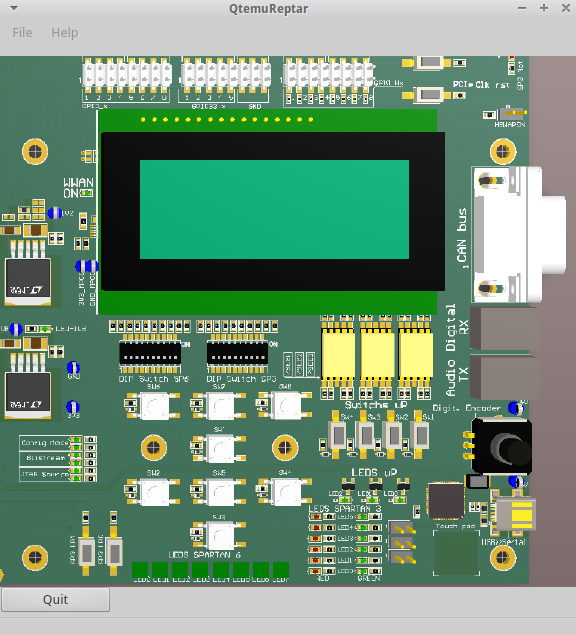
\includegraphics[width=10cm]{img/emulation1.png}
		\caption{Frontend graphique de Qemu}
		\label{emulation1}
	\end{center}
\end{figure}
\textbf{b) Donnée: }Les fichiers sources de Qemu se trouvent dans le répertoire qemu-reds. Examinez les fichiers
suivants :
\begin{enumerate}
	\item hw/arm/reptar/reptar.c Emulation plate-forme REPTAR
	\item hw/reptar\_sp6.c Emulation de la FPGA
	\item hw/reptar\_sp6\_clcd.c Emulation gestion du LCD4x20
	\item hw/reptar\_sp6\_buttons.c Emulation gestion des boutons
	\item hw/reptar\_sp6\_emul.c Gateway entre Qemu et Qtemu
\end{enumerate}
Vous trouverez également toute la documentation nécessaire sur la plate-forme Reptar dans le
répertoire doc. \\\\
\textbf{Remarque: }Ces différents fichiers implémentent ce qui ressemble à des modules noyaux.\\\\
\textbf{c) Donnée: } La compilation de Qemu pourra s'effectuer dans le répertoire qemu-reds directement, avec la
commande make (utilisez make -j4 ou -j8 pour aller plus vite !). \\\\
\textbf{Travail réalisé: }Par la suite, seule la commande \textit{make} sera nécessaire pour recompiler l'émulateur.\\
En lançant \textit{./qtemu} et Eclipse, on pourra debugger l'émulateur Qemu.
\begin{lstlisting}
redsuser@vm-reds-2015s2:~/seee_student$ cd qemu-reds/
redsuser@vm-reds-2015s2:~/seee_student/qemu-reds$ ./configure --target-list=arm-softmmu --enable-debug --disable-attr --disable-docs 
...
redsuser@vm-reds-2015s2:~/seee_student$ make -j8
...
redsuser@vm-reds-2015s2:~/seee_student$
\end{lstlisting}
\subsection{Émulation de la FPGA Spartan6}
Dans cette étape, il s'agit de mettre en place la structure nécessaire à l'émulation de la FPGA intégrée
à la plate-forme. La FPGA implémente des registres associés aux périphériques externes. Dans cette
étape, il s'agit de s'assurer que l'accès aux adresses I/O en lecture et écriture fonctionne. \\\\
\textbf{a) Donnée: }Complétez l'émulation de la FPGA afin de tester l'écriture et la lecture à l'une ou l'autre adresse
dédiée à la FPGA (affichez simplement un message). \\\\
\textbf{Emplacement du code:}\\\textit{/emulationSpartan6\_part2/reptar\_sp6.c}\\ \textit{/emulationSpartan6\_part2/reptar.c}\\\\
\textbf{Travail réalisé: }Nous avons modifié les fichiers \textit{reptar\_sp6.c} et \textit{reptar.c}\\
Le point crucial de cette partie du labo a été de trouvé l'adresse de base de la FPGA qui est \textbf{0x18000000}. Nous avons en effet besoin de cette adresse pour instancier le \textit{reptar\_sp6} dans la partie reptar. 
\begin{lstlisting}
	sysbus_create_simple("reptar_sp6",0x18000000,NULL);
\end{lstlisting}
Pour le reste de l'implémentation, nous nous somme basé sur le diagramme de séquence du support de cours et avons pris le document \textit{versatilepb.c} comme exemple pour le contenu des méthodes callback.\\
Le bon fonctionnement du code a été "testé" premièrement en réussissant la compilation sans erreurs, puis le lancement sans crash. Nous avons également ajouté des messages affichés dans la console dans les différentes méthodes callback pour suivre l'initialisation. L'exécution a été faite de la manière suivante:
\begin{lstlisting}
redsuser@vm-reds-2015s2:~$ cd seee_student/qemu-reds/
redsuser@vm-reds-2015s2:~/seee_student/qemu-reds$ make
...
redsuser@vm-reds-2015s2:~/seee_student/qemu-reds$ cd ..
redsuser@vm-reds-2015s2:~/seee_student$ ./stq
...
sp6 init
reptar-sp6-emul: sp6_emul_init
sp6 initfn
...
Reptar # 
\end{lstlisting}
\textbf{b) Donnée: }Testez les accès en lecture-écriture avec U-Boot. \\\\
\textbf{Travail réalisé: } Pour l'instant, les callback de lecture/écriture que nous avons implémentés contiennent uniquement des messages d'indication qui sont affichés dans la console. À l'aide des commandes suivantes, nous avons pu en tester le bon fonctionnement. Les commandes tentent de lire, puis écrire à l'adresse de la FPGA.
\begin{lstlisting}
Reptar # md.l 0x18000000 1
18000000:sp6 read
 00000000    ....
Reptar # mw.l 0x18000000 1
sp6 write
Reptar #
\end{lstlisting}
\subsection{Émulation des devices de type LED (output)}
\textbf{Donnée: }La FPGA est connectée à des LEDs qui sont visibles sur l'interface graphique. Cette étape consiste à
implémenter le code d'émulation précédent afin de gérer l'accès aux LEDs reliées à la FPGA.
Les interactions entre la FPGA et l'interface graphique doivent être gérées proprement. \\\\
\textbf{Emplacement du code:}\\\textit{/emulationSpartan6\_part3/reptar\_sp6.c}\\\\
\textbf{Travail réalisé: }Pour cette partie, il a fallu rechercher l'offset du registre des LEDs qui est \textit{0x003A}. Il faut donc ajouter cet offset à l'adresse de base de la FPGA. Nous avons défini une variable qui garde la valeur écrite au registre des LEDs pour permettre la relecture de la valeur. La valeur lue est simplement affichée dans la console. Nous avons ensuite implémenté la lecture et l'écriture de ce registre. Pour cela, on teste si l'offset correspond et si l'on lit/écrit des données de la bonne taille, soit 16bits. Des messages ont été implémentés pour indiquer lorsque si la lecture/écriture est faite correctement.
\\Nous avons ensuite testé le bon fonctionnement du code avec le test 10 de itbok. Le test montre que l'on arrive à lire et écrire correctement sur les leds.
\begin{figure}[H]
	\begin{center}
		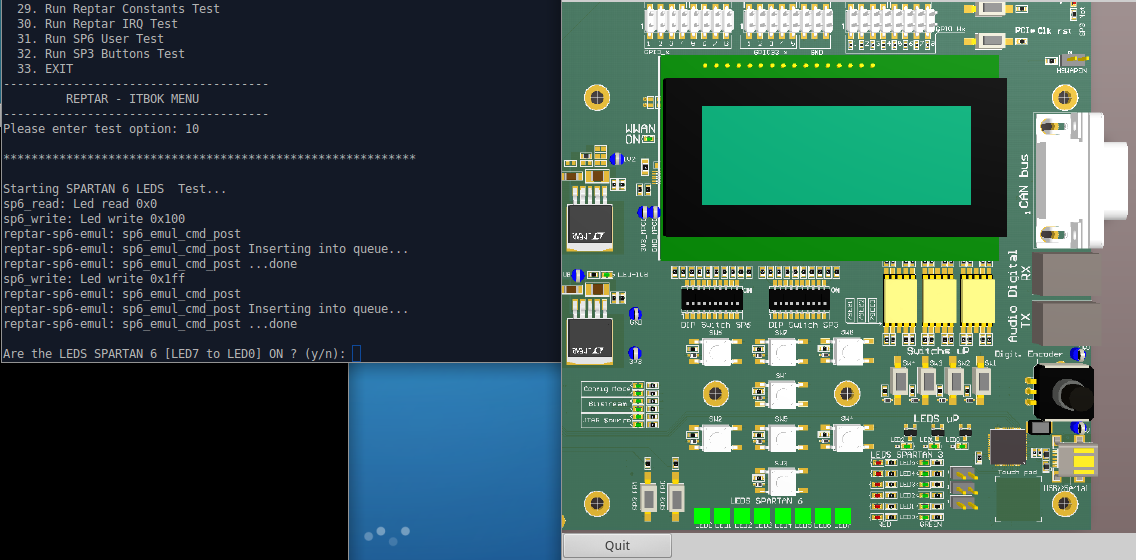
\includegraphics[width=17cm]{img/leds1.png}
		\caption{Test d'allumage des LEDs}
		\label{leds1}
	\end{center}
\end{figure}
\begin{figure}[H]
	\begin{center}
		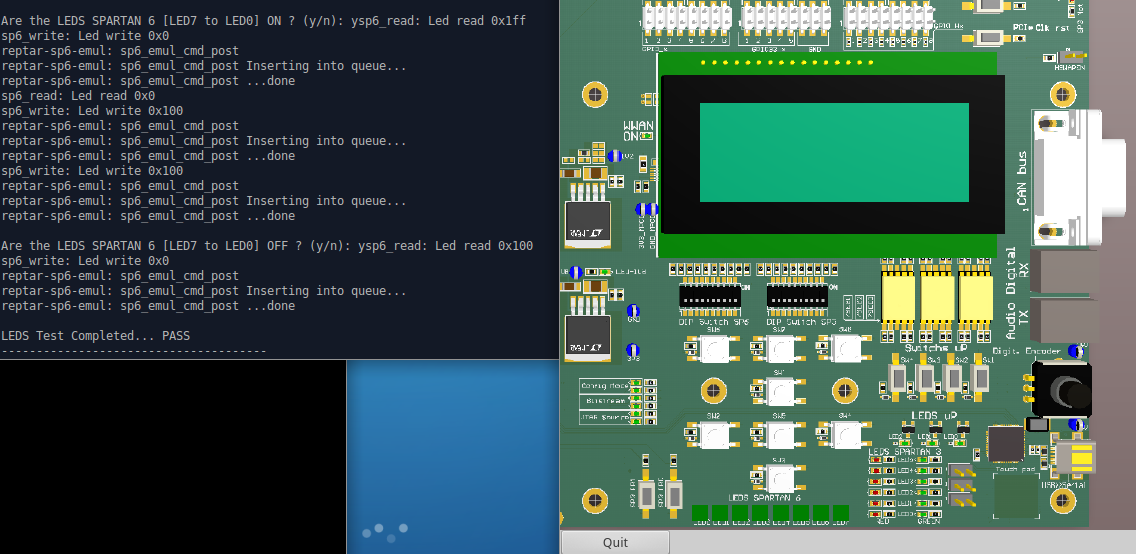
\includegraphics[width=17cm]{img/leds2.png}
		\caption{Test d'extinction des LEDs}
		\label{leds2}
	\end{center}
\end{figure}
\subsection{Émulation de type boutons (input)}
La FPGA est connectée à une série de boutons (switches) sur la plate-forme Reptar. Cette étape consiste
à mettre en place la structure nécessaire à la gestion de ces boutons. \\\\
\textbf{a) Donnée: }Adaptez les fichiers nécessaires afin que l'émulation de votre périphérique (FPGA) puisse détecter
la pression d'une touche, sans vous préoccuper pour le moment des interruptions. \\\\
\textbf{Emplacement du code:}\\\textit{/emulationSpartan6\_part4/reptar\_sp6.c}\\
\textit{/emulationSpartan6\_part4/reptar\_sp6\_buttons.c}\\\\
\textbf{Travail réalisé: }Le code de cette partie est inspiré du \textit{Guide d'utilisation de l'infrastructure}. L'offset pour lire la valeur des boutons est \textit{0x0012}. Lorsqu'un bouton est pressé, le handler du fichier sp6\_button est appelé et la valeur du registre est mémorisée. La valeur des boutons peut également être récupérée lors d'une lecture du registre \textit{0x0012}.\\\\
\textbf{b) Donnée: }Le projet sp6\_buttons\_u-boot contient une application permettant de tester vos boutons (en mode
polling). Compilez l'application et effectuez quelques tests.\\\\
\textbf{Travail réalisé: }L'application a été compilée avec make. Il faut ensuite lancer l'émulateur avec la \textit{stq}. Une fois dans l'U-boot, on peut lancer l'application testant les boutons facilement, car elle est enregistrée dans les variables d'environnements sous le nom \textit{tftp3}. Les lignes ci-dessous démontre le bon fonctionnement des boutons. Le bouton exit arrête l'application. 
\begin{lstlisting}
redsuser@vm-reds-2015s2:~/seee_student$ ./stq
...
Reptar # run tftp3
smc911x: detected LAN9118 controller
smc911x: phy initialized
smc911x: MAC e4:af:a1:40:01:fe
Using smc911x-0 device
TFTP from server 10.0.2.2; our IP address is 10.0.2.10
Filename 'sp6_buttons_u-boot/sp6_buttons.bin'.
Load address: 0x81600000
Loading: #######
done
Bytes transferred = 34512 (86d0 hex)

Reptar # run goapp
## Starting application at 0x81600000 ...
Start of the SP6 buttons standalone test application.
Button ONE pressed
...
Button ONE pressed
Button ONE pressed
Button ONE pressed
reptar-sp6-emul: sp6_emul_event_handle: read 29 
reptar-sp6-emul: sp6_emul_event_handle: cJSON_Parse done 
Button status : 0x0

Button LEFT pressed
Button LEFT pressed
Button LEFT pressed
reptar-sp6-emul: sp6_emul_event_handle: read 29 
reptar-sp6-emul: sp6_emul_event_handle: cJSON_Parse done 
Button status : 0x0

reptar-sp6-emul: sp6_emul_event_handle: read 30 
reptar-sp6-emul: sp6_emul_event_handle: cJSON_Parse done 
Button status : 0x10
Button EXIT pressed
SP6 buttons standalone test application exit.
## Application terminated, rc = 0x0
Reptar # reptar-sp6-emul: sp6_emul_event_handle: read 29 
reptar-sp6-emul: sp6_emul_event_handle: cJSON_Parse done 
Button status : 0x0
\end{lstlisting}
\subsection{Gestion des interruptions (IRQ) avec les boutons}
Complétez votre émulateur avec le code nécessaire à la gestion d'une interruption à niveau émise par
la FPGA lorsqu'un bouton est pressé. L'interruption est censée être acquittée par le driver. Il faut donc
gérer l'état interne associé à cette interruption. \\\\
\textbf{a) Donnée: }Commencez par adapter le code d'initialisation de la plate-forme (reptar.c) afin d'instancier une
interruption en provenance de la FPGA ; l'interruption sera de type niveau.\\\\
\textbf{Travail réalisé: }\\\\
\textbf{b) Donnée: }Testez que l'interruption fonctionne en configurant le contrôleur GPIO et en interrogeant le registre
d'état, dans U-Boot. Les registres du microcontrôleur à utiliser sont les suivants :
GPIO\_RISINGDETECT, GPIO\_IRQENABLE1 et GPIO\_IRQSTATUS1
De plus, l'interruption doit aussi être activée au niveau de la FPGA (cf documentation). \\\\
\textbf{Travail réalisé: }\\\\
\subsection{Émulation de l'afficheur 7 segments}
La FPGA est connectée à un afficheur 7 segments, visible sur l’émulateur. Cette étape consiste à mettre
en place la gestion de cet afficheur 7 segments.\\\\
\textbf{a) Donnée: }Adaptez les fichiers nécessaires afin que l'émulation de votre périphérique (FPGA) puisse gérer les
trois digits de l’afficheur 7 segments. \\\\
\textbf{Emplacement du code:}\textit{/emulationSpartan6\_part6/reptar\_sp6.c}\\\\
\textbf{Travail réalisé: }Pour cette partie, nous avons simplement ajouté le code pour écrire et lire dans le registre de chacun des trois digits de l'affichage 7 segments. La valeur de chaque affichage est stocké dans une variable. Pour l'écriture, il faut spécifier dans le gson le nom du périphérique, le numéro du digit ainsi que la valeur à afficher.\\\\
\textbf{b) Donnée: }Le dossier 7seg\_u-boot contient une application permettant de tester l’afficheur 7 segments : les
chiffres de 0 à 9 doivent défiler progressivement : 012, puis 123, 234, 456, 567, …, 901, 012, etc.
Compilez l'application et effectuez quelques tests.\\\\
\textbf{Travail réalisé: }Une fois l'application compilée, il a fallu la lancer dans l'U-boot. Comme elle n'est pas définie dans les variables d'environnement, il faut utiliser la commande complète. Une fois lancée, l'application va incrémenter la valeur des digits. L'image ci-dessous démontre le bon fonctionnement.
\begin{lstlisting}
redsuser@vm-reds-2015s2:~/seee_student$ ./stq
...
Reptar # tftp 7seg_u-boot/7seg_u-boot.bin
smc911x: detected LAN9118 controller
smc911x: phy initialized
smc911x: MAC e4:af:a1:40:01:fe
Using smc911x-0 device
TFTP from server 10.0.2.2; our IP address is 10.0.2.10
Filename '7seg_u-boot/7seg_u-boot.bin'.
Load address: 0x81600000
Loading: #######
done
Bytes transferred = 34932 (8874 hex)
Reptar # run goapp
\end{lstlisting}
\begin{figure}[H]
	\begin{center}
		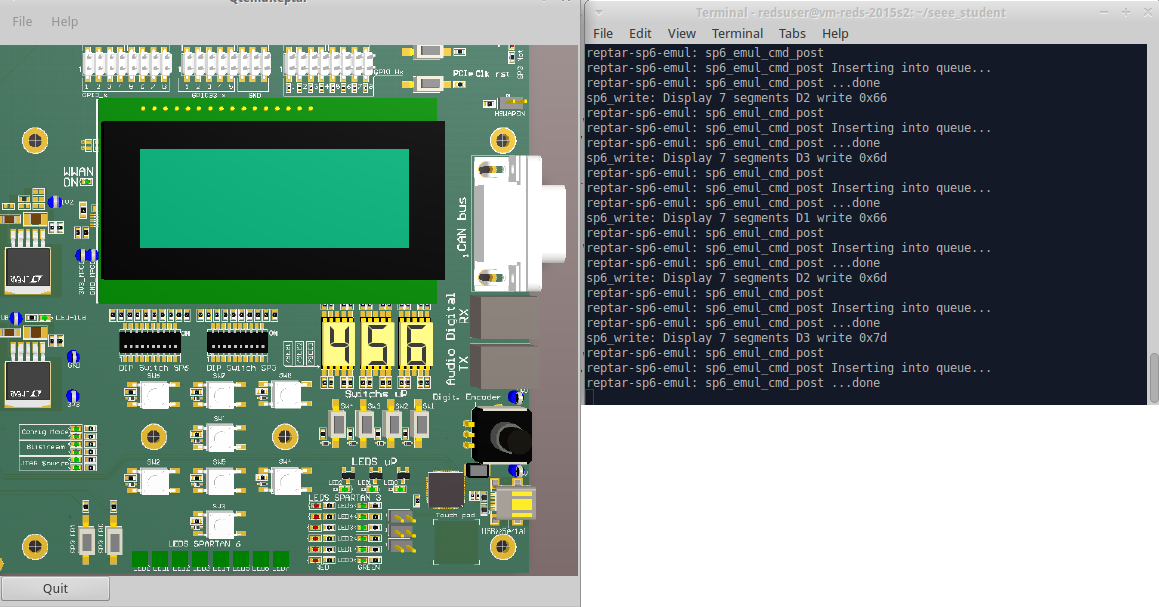
\includegraphics[width=15cm]{img/emulation2.png}
		\caption{Frontend graphique de Qemu avec affichage 7 segments}
		\label{emulation2}
	\end{center}
\end{figure}
\subsection{Mini-application utilisant les boutons et l'afficheur 7 segments}
\textbf{a) Donnée: }Le dossier miniapp\_u-boot contient un chablon. Complétez-le afin de créer une application qui
utilise les boutons SW2, SW5, SW4 et SW3, ainsi que l’afficheur 7 segments.
\begin{enumerate}
	\item Lors d’un appui sur SW2, SW5 ou SW4, le digit respectivement à gauche, au centre ou au
	milieu est incrémenté de 1, modulo 10. Si un digit atteint 9, il reviendra à 0. 
	\item La valeur initiale de chaque digit, au démarrage de l’application, est 0 (on affichera 000). 
	\item Un appui sur SW3 quitte l’application. 
	\item Vous devrez gérer l’anti-rebond : le digit ne devra être incrémenté que si le bouton est
	pressé puis relâché (comme un appui sur une touche de sonnette par exemple). \\
\end{enumerate}
\textbf{Travail réalisé: }\\\\
\textbf{b) Donnée: }Testez votre application sur l’émulateur\\\\
\textbf{Travail réalisé: }\\\\
\textbf{c) Donnée: }Déployez et testez votre application sur la plate-forme réelle\\\\
\textbf{Travail réalisé: }\\\\


